\begin{figure}[htbp]
\centering
\begin{tabular}{@{}c@{\hspace{10mm}}c@{}}
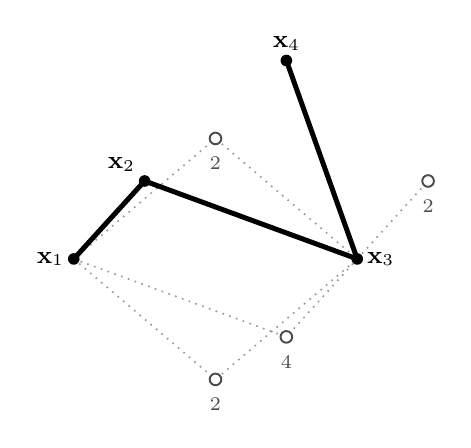
\begin{tikzpicture}[baseline]
  \draw[dotted,black!40,line width=0.6pt] (0.000,0.000) -- (2.700,-0.990) -- (3.600,0.000);
  \draw[dotted,black!40,line width=0.6pt] (0.000,0.000) -- (1.800,1.530) -- (3.600,0.000);
  \draw[dotted,black!40,line width=0.6pt] (0.000,0.000) -- (1.800,-1.530) -- (3.600,0.000);
  \draw[dotted,black!40,line width=0.6pt] (3.600,0.000) -- (4.500,0.990);
  \draw[line width=1.8pt,black] (0.000,0.000) -- (0.900,0.990) -- (3.600,0.000) -- (2.700,2.520);
  \fill[white] (2.700,-0.990) circle (2.1pt); \draw[black!70,line width=0.7pt] (2.700,-0.990) circle (2.1pt);
  \node[font=\scriptsize,black!70] at (2.700,-1.310) {4};
  \fill[white] (1.800,1.530) circle (2.1pt); \draw[black!70,line width=0.7pt] (1.800,1.530) circle (2.1pt);
  \node[font=\scriptsize,black!70] at (1.800,1.210) {2};
  \fill[white] (1.800,-1.530) circle (2.1pt); \draw[black!70,line width=0.7pt] (1.800,-1.530) circle (2.1pt);
  \node[font=\scriptsize,black!70] at (1.800,-1.850) {2};
  \fill[white] (4.500,0.990) circle (2.1pt); \draw[black!70,line width=0.7pt] (4.500,0.990) circle (2.1pt);
  \node[font=\scriptsize,black!70] at (4.500,0.670) {2};
  \fill[black] (0.000,0.000) circle (2.1pt);
  \fill[black] (0.900,0.990) circle (2.1pt);
  \fill[black] (3.600,0.000) circle (2.1pt);
  \fill[black] (2.700,2.520) circle (2.1pt);
  \node[anchor=east,font=\small] at (0.000,0.000) {$\mathbf x_1$};
  \node[anchor=south east,font=\small] at (0.900,0.990) {$\mathbf x_2$};
  \node[anchor=west,font=\small] at (3.600,0.000) {$\mathbf x_3$};
  \node[anchor=south,font=\small] at (2.700,2.520) {$\mathbf x_4$};
\end{tikzpicture}
&
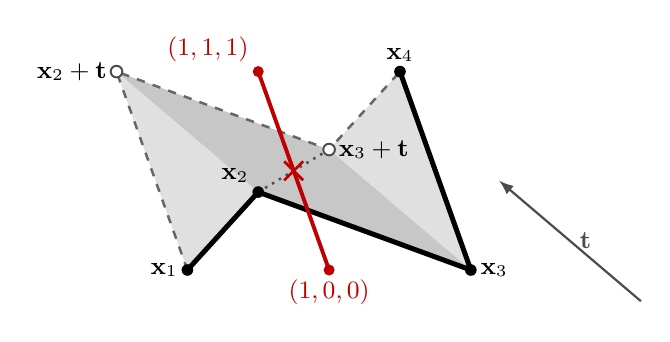
\begin{tikzpicture}[baseline]
  \fill[black!12] (0.000,0.000) -- (0.900,0.990) -- (-0.900,2.520) -- cycle;
  \fill[black!12] (2.700,2.520) -- (3.600,0.000) -- (1.800,1.530) -- cycle;
  \fill[black!22] (0.900,0.990) -- (3.600,0.000) -- (1.800,1.530) -- (-0.900,2.520) -- cycle;
  \draw[dashed,black!60,line width=0.9pt] (0.000,0.000) -- (-0.900,2.520) -- (1.800,1.530) -- (2.700,2.520);
  \draw[dotted,black!70,line width=0.9pt] (0.900,0.990) -- (1.800,1.530);
  \draw[line width=1.8pt,black] (0.000,0.000) -- (0.900,0.990) -- (3.600,0.000) -- (2.700,2.520);
  \draw[line width=1.4pt,red!75!black] (1.800,0.000) -- (0.900,2.520);
  \fill[red!75!black] (1.800,0.000) circle (2.0pt); \fill[red!75!black] (0.900,2.520) circle (2.0pt);
  \draw[red!75!black,line width=1.0pt] (1.230,1.140) -- (1.470,1.380) (1.230,1.380) -- (1.470,1.140);
  \fill[white] (-0.900,2.520) circle (2.1pt); \draw[black!70,line width=0.7pt] (-0.900,2.520) circle (2.1pt);
  \fill[white] (1.800,1.530) circle (2.1pt); \draw[black!70,line width=0.7pt] (1.800,1.530) circle (2.1pt);
  \fill[black] (0.000,0.000) circle (2.1pt);
  \fill[black] (0.900,0.990) circle (2.1pt);
  \fill[black] (3.600,0.000) circle (2.1pt);
  \fill[black] (2.700,2.520) circle (2.1pt);
  \node[anchor=east,font=\small] at (0.000,0.000) {$\mathbf x_1$};
  \node[anchor=south east,font=\small] at (0.900,0.990) {$\mathbf x_2$};
  \node[anchor=west,font=\small] at (3.600,0.000) {$\mathbf x_3$};
  \node[anchor=south,font=\small] at (2.700,2.520) {$\mathbf x_4$};
  \node[anchor=east,font=\small] at (-0.900,2.520) {$\mathbf x_2+\mathbf t$};
  \node[anchor=west,font=\small] at (1.800,1.530) {$\mathbf x_3+\mathbf t$};
  \node[anchor=north,font=\small,red!75!black] at (1.800,0.000) {$(1,0,0)$};
  \node[anchor=south east,font=\small,red!75!black] at (0.900,2.520) {$(1,1,1)$};
  \draw[-latex,black!70,line width=0.8pt] (5.760,-0.396) -- (3.960,1.134);
  \node[anchor=west,font=\small,black!70] at (4.860,0.369) {$\mathbf t$};
\end{tikzpicture}
\\[1mm]
{\footnotesize (a) kink and end rotation} & {\footnotesize (b) edge translation of a segment} \\
\end{tabular}
\caption{The moves of \Cref{sec:fcc-moveset} acting on a four-unit chain. 
(a) Units $\mathbf x_1\ldots\mathbf x_4$; the three kink destinations of
$\mathbf x_2$ and one end-bond rotation of $\mathbf x_4$ are open circles labeled by their squared
chord length in units of $h^2$, and the dotted lines are the new bonds. (b) The segment
$\{\mathbf x_2,\mathbf x_3\}$ carried by the edge vector $\mathbf t=(-1,0,1)$ to the open circles.
The anchor bonds sweep the two lighter equilateral triangles and the internal bond the darker
rhombus, whose short diagonal is the dotted segment from $\mathbf x_2$ to $(1,0,1)$. The red bond
is an example of a bond that is of an opposite parity class and crosses that diagonal at its midpoint, the point marked; it
is the single read the translation needs when both classes are present, and it is also the bond that
would refuse the sideways kink $\mathbf x_2\to(1,0,1)$ of panel (a).}
\label{fig:si-fccmoves}
\end{figure}
